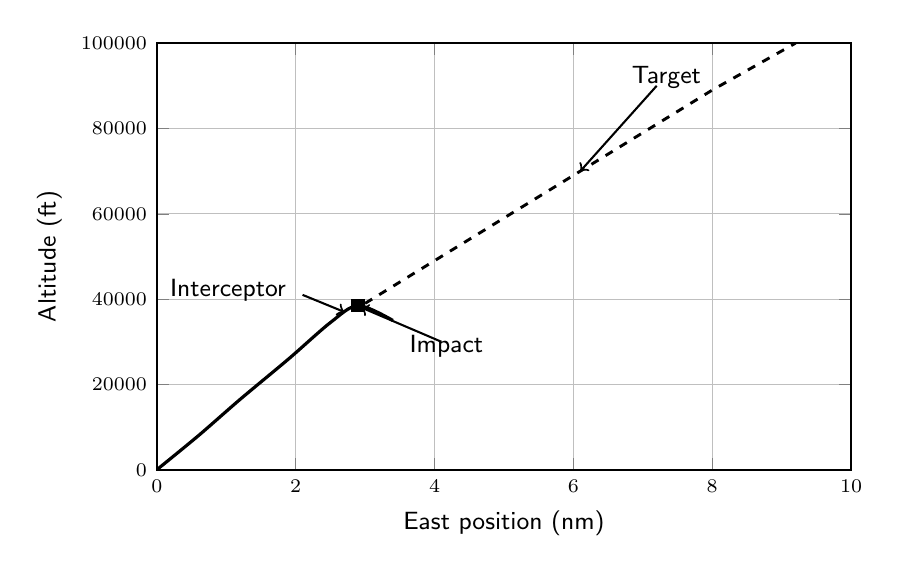
\begin{tikzpicture}
\begin{axis}[
  width=10.4cm,height=7.0cm,
  xmin=0,xmax=10,ymin=0,ymax=100000,
  xtick={0,2,4,6,8,10},
  ytick={0,20000,40000,60000,80000,100000},
  grid=major,
  axis line style={line width=0.8pt},
  tick label style={font=\scriptsize},
  label style={font=\sffamily\small},
  xlabel={East position (nm)},ylabel={Altitude (ft)},
  scaled y ticks=false,
  yticklabel style={/pgf/number format/fixed,/pgf/number format/1000 sep={}},
]
  \addplot[line width=1.15pt,smooth] coordinates {(0,0) (0.6,8000) (1.2,16500) (1.9,26000) (2.5,34500) (2.9,38500) (3.4,35000)};
  \addplot[line width=1.05pt,dashed] coordinates {(3.0,39000) (4.2,51000) (5.5,64000) (6.8,77000) (8.0,89000) (9.2,100000)};
  \addplot[only marks,mark=square*,mark size=2.2pt] coordinates {(2.9,38500)};
  \node[font=\sffamily\small,anchor=east] at (axis cs:2.0,42000) {Interceptor};
  \draw[->,line width=0.75pt] (axis cs:2.1,41000)--(axis cs:2.7,37000);
  \node[font=\sffamily\small,anchor=west] at (axis cs:6.7,92000) {Target};
  \draw[->,line width=0.75pt] (axis cs:7.2,90000)--(axis cs:6.1,70000);
  \node[font=\sffamily\small,anchor=west] at (axis cs:3.5,29000) {Impact};
  \draw[->,line width=0.75pt] (axis cs:4.1,30000)--(axis cs:2.95,38000);
\end{axis}
\end{tikzpicture}
